\documentclass[12pt,a4paper,hidelinks]{article}

\usepackage{ulem}
\usepackage{incgraph}
\usepackage{tikz}
\usepackage{hyperref}

\newcommand{\leftcoordinate}{-15cm}
\usetikzlibrary{mindmap,shadows,calendar,fadings}
\tikzset{todo/.append style={annotation,above,concept color=white,draw=black,text width=2cm,align=center}}
\hypersetup{
    colorlinks=false,
    linkcolor=black,
    filecolor=magenta,      
    urlcolor=cyan,
}

\begin{document}
\begin{inctext}
    \begin{tikzpicture}
        \pgfdeclarelayer{background}
        \pgfdeclarelayer{foreground}
        \pgfsetlayers{background,main,foreground}
        % ------------------------ declare mindmap ------------------------ %
        \begin{scope}[
                mindmap,
                grow cyclic,
                concept color=pink,
                every node/.append style={concept,circular drop shadow,text width=4cm},
                level 1/.append style={sibling angle=360/5},
                every child/.append style={level distance=7cm,font=\fontsize{10pt}{12pt}}
            ]
            \node[root concept, fill=white](isa){
                \href{https://www.youtube.com/watch?v=PlavjNH_RRU&list=PLylNWPMX1lPlmEeeMdbEFQo20eHAJL8hx&index=1}{Introduction to ISA}
            }
            child[concept color=gray]{
                    node{
                            \href{https://stackoverflow.com/questions/54910933/difference-between-store-word-load-word-and-move}{Load word, Store word}
                        }
                };
            \node[fill=white,yshift=10cm](instruction){
                \href{https://www.youtube.com/watch?v=SFv_QaNFshk&list=PLylNWPMX1lPlmEeeMdbEFQo20eHAJL8hx&index=4}{Instruction Execution Model}
            }
            child{
                    node{
                            \href{https://www.cloudflare.com/learning/security/threats/buffer-overflow/}{What is buffer overflow?}
                        }
                }
            child{
                    node{
                            \href{https://www.imperva.com/learn/application-security/buffer-overflow/}{What is buffer overflow 2}
                        }
                }
            child{
                    node(overflow){
                            \href{https://www.youtube.com/watch?v=1S0aBV-Waeo}{Running a Buffer Overflow Attack}
                        }
                }
            ;
        \end{scope}
        % ------------------------ background ------------------------ %
        \begin{pgfonlayer}{background}

        \end{pgfonlayer}
        % ------------------------ foreground ------------------------ %
        \begin{pgfonlayer}{foreground}
            \node[text width=1.5cm, text height=1.5cm,yshift=-1.1cm] at (isa) {
                \href{https://www.youtube.com/watch?v=PlavjNH_RRU&list=PLylNWPMX1lPlmEeeMdbEFQo20eHAJL8hx&index=1}{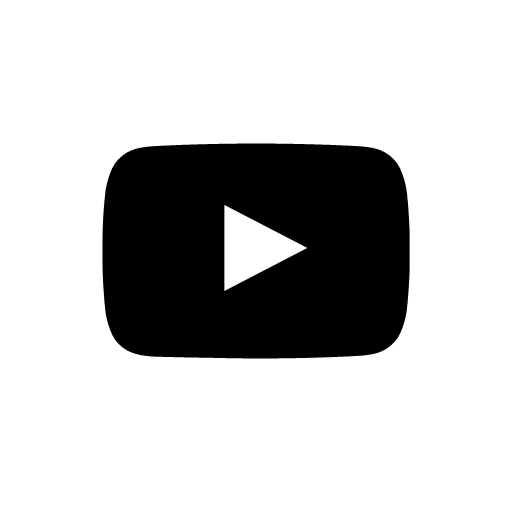
\includegraphics[width=1.5cm,height=1.5cm]{./image/youtube.png}}
            };
            \node[text width=1.5cm, text height=1.5cm,yshift=-1.1cm] at (instruction) {
                \href{https://www.youtube.com/watch?v=PlavjNH_RRU&list=PLylNWPMX1lPlmEeeMdbEFQo20eHAJL8hx&index=1}{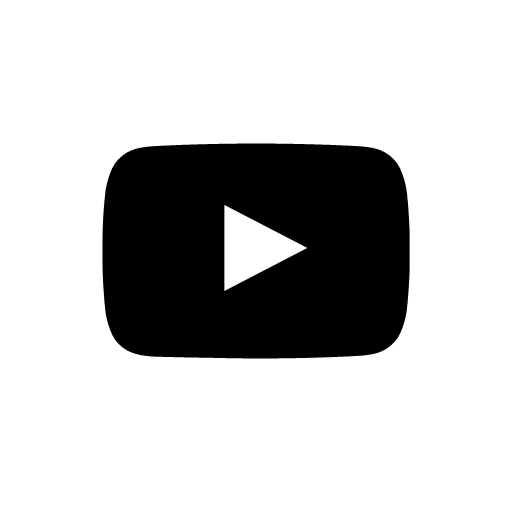
\includegraphics[width=1.5cm,height=1.5cm]{./image/youtube.png}}
            };
            \node[text width=1.5cm, text height=1.5cm,yshift=-1.1cm] at (overflow) {
                \href{https://www.youtube.com/watch?v=1S0aBV-Waeo}{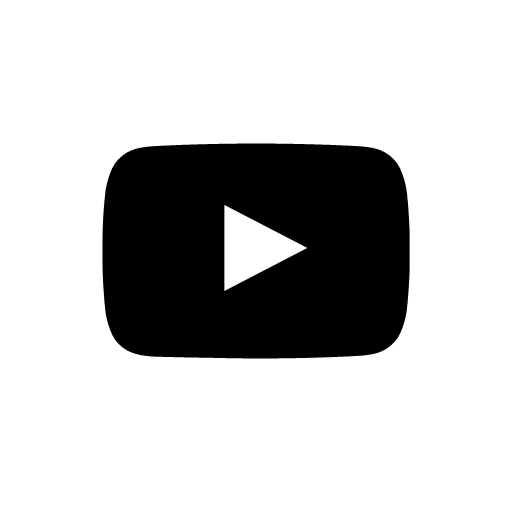
\includegraphics[width=1.5cm,height=1.5cm]{./image/youtube.png}}
            };
        \end{pgfonlayer}
    \end{tikzpicture}
\end{inctext}
%------------------------------------------------------------ List ------------------------------------------------------------%
\noindent
1. Should add useful and understandable documents\\
\end{document}